\documentclass{beamer}

\usepackage{amsmath}
\usepackage{booktabs} % Para tabelas com visual profissional
\usepackage{tabularx} % Para tabelas com largura definida e colunas do tipo X


\usetheme{Madrid}
\usecolortheme{beaver}
\usepackage[utf8]{inputenc}
\usepackage[brazil]{babel}
\usepackage{graphicx}
\usepackage{xcolor}
\usepackage{colortbl} % para sombrear células da tabela
\usepackage{tikz}
%\usetikzlibrary{shapes, arrows.meta, positioning}
\usetikzlibrary{shapes.geometric, arrows.meta, positioning, calc, decorations.pathreplacing}

\usepackage{array}

\usepackage{tcolorbox}     % Para caixas coloridas e formatadas
\tcbuselibrary{skins, breakable}  % Habilita opções avançadas do tcolorbox
\usepackage{graphicx}      % Necessário para \scalebox
\usepackage{hyperref}
\hypersetup{
    colorlinks=true,
    %linkcolor=blue,
    filecolor=magenta,
    urlcolor=cyan,
    pdfpagemode=FullScreen,
    }

\urlstyle{same}


\definecolor{graycell}{gray}{0.85} % define a cor de fundo da célula
\definecolor{vermelhoClaro}{RGB}{255, 200, 200}


\AtBeginSection[]
{
  \begin{frame}
    \frametitle{Índice}
    \tableofcontents[currentsection]
  \end{frame}
}

%% Placeholder para figuras ainda não disponíveis: se o arquivo existir em img/,
%% inclui a imagem; senão desenha uma caixa indicando qual figura do livro buscar.
%% Uso: \figuraplaceholder[largura]{img/arquivo.png}{Fig. X.Y do livro (pág. Z)}
\newcommand{\figuraplaceholder}[3][0.8\textwidth]{%
    \IfFileExists{#2}{%
        \includegraphics[width=#1]{#2}%
    }{%
        \begin{tikzpicture}
            \node[draw=gray!70, dashed, very thick, fill=gray!10,
                  minimum width=0.85\textwidth, minimum height=2.6cm, align=center]
                {{\large\bfseries\color{gray!60!black} PLACEHOLDER}\\[3pt]
                 #3\\[3pt]
                 {\footnotesize arquivo esperado: \texttt{#2}}};
        \end{tikzpicture}%
    }%
}

% Informações da apresentação
\title[MACs]{Códigos de Autenticação de Mensagem (MACs)}
\author{Prof. Iaçanã Ianiski Weber}
\institute{PUCRS}
\date{CSS (98G08-4)}

\begin{document}

% Slide de Capa Personalizado
\begin{frame}[plain]

% Linha superior com logo e título
\noindent
\begin{minipage}[t]{0.15\textwidth}
    
\includegraphics[width=\linewidth]{img/Brasão_PUCRS.png}
\end{minipage}%
\begin{minipage}[t]{0.84\textwidth}
    \begin{center}
        {\LARGE\bfseries\textcolor{blue}{Código de Autenticação\\[2pt] de Mensagem (MACs)}}
    \end{center}
\end{minipage}

\vspace{2cm}

\begin{center}
    \Large \textbf{Prof. Dr. Iaçanã Ianiski Weber} \\
    \vspace{0.2cm}
    \normalsize \textit{Confiabilidade e Segurança de Software} \\
    \vspace{0.2cm}
    \large 98G08-4
\end{center}

\vfill

\begin{center}
    \tiny \textit{Agradecimentos especiais ao Prof. Avelino Zorzo e aos Autores Christof Paar e Jan Pelzl pelo material.}
\end{center}

\end{frame}

% Slide de Índice
\begin{frame}{Índice}
    \tableofcontents
\end{frame}

\begin{frame}{Conteúdo deste Capítulo}
    \vspace{0.5em}
    Nesta aula você vai aprender:
    \begin{itemize}
        \item O \textbf{princípio} por trás dos MACs (\textit{Message Authentication Codes}).
        \medskip
        \item As \textbf{propriedades de segurança} que os MACs oferecem, e a que eles \textbf{não} oferecem (não repúdio).
        \medskip
        \item Como MACs podem ser construídos a partir de \textbf{funções hash} (\textbf{HMAC} e \textbf{KMAC}).
        \medskip
        \item Como MACs podem ser construídos a partir de \textbf{cifras de bloco} (\textbf{CBC-MAC} e \textbf{CMAC}).
        \medskip
        \item Como combinar \textbf{confidencialidade + autenticação} em um único passo: \textbf{encriptação autenticada} (\textbf{CCM}, \textbf{GCM}, \textbf{GMAC}).
    \end{itemize}
\end{frame}

%%%%%%%%%%%%%%%%%%%%%%%%%%%%%%%%%%%
%%%%%%%%%%%%%%%%%%%%%%%%%%%%%%%%%%%
%%%%%%%%%%%%%%%%%%%%%%%%%%%%%%%%%%%
\section{Por que Precisamos de MACs}

\begin{frame}{Motivação: Integridade e Autenticação}
    \textbf{O problema:} Bob envia uma mensagem $x$ a Alice por um canal inseguro. Como Alice tem certeza de que:
    \begin{itemize}
        \item a mensagem \alert{não foi alterada} no caminho (\textbf{integridade}); e
        \item a mensagem realmente \alert{veio de Bob} (\textbf{autenticação de origem})?
    \end{itemize}
    \bigskip\pause
    \textbf{Por que um hash sozinho não basta?}
    \begin{itemize}
        \footnotesize
        \item Funções hash são \textbf{sem chave} (\textit{keyless}): \emph{qualquer um} pode calcular $h(x)$.
        \item Se Bob enviasse $(x, h(x))$, o atacante Oscar poderia trocar a mensagem por $x'$ e simplesmente recalcular $h(x')$. Alice não perceberia.
        \item \textbf{Falta um segredo} que ligue a mensagem a quem a produziu.
    \end{itemize}
    \bigskip\pause
    \textbf{A ideia do MAC:} introduzir uma \textbf{chave secreta simétrica $k$}, compartilhada entre Bob e Alice, no cálculo do ``checksum''. Só quem tem $k$ consegue gerar uma \textit{tag} válida.
\end{frame}

\begin{frame}{Onde os MACs se Encaixam}
    Três ferramentas que produzem uma ``etiqueta'' a partir de uma mensagem:
    \medskip
    \begin{center}
        \small
        \begin{tabular}{lccc}
            \toprule
            & \textbf{Função Hash} & \textbf{MAC} & \textbf{Assinatura Digital} \\
            \midrule
            Usa chave?            & \cellcolor{red!12}Não (keyless) & \cellcolor{green!12}Simétrica & \cellcolor{green!12}Assimétrica \\
            Integridade           & \cellcolor{green!12}Sim$^\ast$ & \cellcolor{green!12}Sim & \cellcolor{green!12}Sim \\
            Autenticação de origem& \cellcolor{red!12}Não & \cellcolor{green!12}Sim & \cellcolor{green!12}Sim \\
            Não repúdio           & \cellcolor{red!12}Não & \cellcolor{red!12}\alert{Não} & \cellcolor{green!12}Sim \\
            Velocidade            & \cellcolor{green!12}Rápida & \cellcolor{green!12}Rápida & \cellcolor{red!12}Lenta \\
            \bottomrule
        \end{tabular}
    \end{center}
    \medskip
    \begin{itemize}
        \footnotesize
        \item[$\ast$] O hash detecta alterações \emph{acidentais}, mas não \emph{maliciosas} se enviado sem proteção.
        \item \textbf{O MAC é o ``meio-termo''}: oferece integridade \emph{e} autenticação como a assinatura, mas com o desempenho da criptografia simétrica.
        \item \textbf{Preço a pagar:} como a chave é \emph{compartilhada}, o MAC \alert{não fornece não repúdio} (veremos por quê).
    \end{itemize}
\end{frame}

%%%%%%%%%%%%%%%%%%%%%%%%%%%%%%%%%%%
\section{Princípios dos MACs}

\begin{frame}{Princípio dos MACs}
    \begin{itemize}
        \item De forma semelhante às assinaturas digitais, MACs acrescentam uma \textit{tag} de autenticação a uma mensagem.
        \item MACs utilizam uma \textbf{chave simétrica $k$} tanto para a \textbf{geração} quanto para a \textbf{verificação}.
        \item Cálculo de um MAC:
        \[
            m = \text{MAC}_k(x)
        \]
        é uma função da chave secreta $k$ e da mensagem $x$.
    \end{itemize}
    \begin{center}
        \figuraplaceholder[0.62\textwidth]{img/mac_principle.png}{Fig.~13.1 do livro: protocolo básico de proteção de $x$ com um MAC (pág.~466)}
    \end{center}
\end{frame}

\begin{frame}{O Protocolo Passo a Passo}
    \begin{columns}[T]
        \begin{column}{0.5\textwidth}
            \textbf{Bob (remetente):}
            \begin{enumerate}
                \footnotesize
                \item Calcula $m = \text{MAC}_k(x)$ com a chave secreta $k$.
                \item Envia o par $(x, m)$ para Alice.
            \end{enumerate}
            \bigskip
            \textbf{Alice (receptora):}
            \begin{enumerate}
                \footnotesize
                \item Recebe $(x, m)$.
                \item Recalcula $m' = \text{MAC}_k(x)$ com a \emph{mesma} chave $k$.
                \item Verifica se $m' \overset{?}{=} m$.
            \end{enumerate}
        \end{column}
        \begin{column}{0.5\textwidth}
            {\small\textbf{Interpretação do resultado:}}
            \begin{itemize}
                \footnotesize
                \item $m' = m$ $\Rightarrow$ mensagem \textbf{íntegra} e \textbf{autêntica} (só quem tem $k$ poderia ter gerado $m$).
                \item $m' \neq m$ $\Rightarrow$ a mensagem $x$ \emph{e/ou} a \textit{tag} $m$ foram \alert{alteradas} em trânsito.
            \end{itemize}
            \medskip
            \begin{tcolorbox}[colback=blue!5,colframe=blue!50!black,boxrule=0.5pt,left=2pt,right=2pt,top=2pt,bottom=2pt]
                \footnotesize
                \textbf{Premissa fundamental:} se $x$ for alterada em trânsito, o MAC recomputado dará um valor \emph{diferente}. Oscar não consegue forjar $m$ sem conhecer $k$.
            \end{tcolorbox}
        \end{column}
    \end{columns}
\end{frame}

\begin{frame}{Propriedades dos Códigos de Autenticação de Mensagens}
    \begin{enumerate}
        \footnotesize
        \item \textbf{Checksum criptográfico:} um MAC gera uma \textit{tag} de autenticação criptograficamente segura para uma dada mensagem.
        \item \textbf{Simétrico:} MACs são baseados em chaves simétricas secretas. As partes que geram e verificam o MAC devem \emph{compartilhar} uma chave secreta.
        \item \textbf{Tamanho arbitrário de mensagem:} MACs aceitam mensagens de comprimento arbitrário.
        \item \textbf{Comprimento de saída fixo:} MACs geram \textit{tags} de tamanho fixo (independente do tamanho da entrada).
        \item \textbf{Integridade da mensagem:} qualquer modificação na mensagem em trânsito será detectada pelo receptor.
        \item \textbf{Autenticação da mensagem:} a parte que recebe é assegurada quanto à origem legítima da mensagem.
        \item \textbf{Ausência de não repúdio:} como MACs são baseados em princípios simétricos, eles \alert{não} fornecem não repúdio.
    \end{enumerate}
\end{frame}

\begin{frame}{Por que MACs Não Fornecem Não Repúdio?}
    \begin{itemize}
        \item Alice e Bob \textbf{compartilham a mesma chave $k$}.
        \item Logo, \emph{ambos} são capazes de gerar qualquer \textit{tag} válida $m = \text{MAC}_k(x)$.
        \bigskip\pause
        \item Diante de um juiz, é \alert{impossível provar} quem dos dois gerou a mensagem:
        \begin{itemize}
            \footnotesize
            \item Bob pode alegar que foi Alice quem forjou a mensagem (e vice-versa).
            \item A chave simétrica está ligada a \emph{duas} partes, não a \emph{uma} pessoa (ao contrário da chave privada assimétrica).
        \end{itemize}
        \bigskip\pause
        \item \textbf{Conclusão:} MACs não protegem em cenários onde uma das partes pode ser desonesta (ex.: o caso da compra/venda de carro visto em assinaturas digitais).
    \end{itemize}
    \bigskip
    \begin{tcolorbox}[colback=green!5,colframe=green!50!black,boxrule=0.5pt]
        \footnotesize
        \textbf{Quando o não repúdio importa $\Rightarrow$ use assinatura digital.} \quad
        \textbf{Quando importa velocidade entre partes que confiam mutuamente $\Rightarrow$ use MAC.}
    \end{tcolorbox}
\end{frame}

\begin{frame}{Quão Longa Deve Ser a \textit{Tag} de um MAC?}
    \textbf{Diferente das funções hash!} Em um hash, precisamos de saída $\geq 256$ bits para resistir ao \textit{birthday attack}. Em um MAC, \alert{tags de 128 bits costumam bastar}. Por quê?
    \medskip
    \begin{itemize}
        \footnotesize
        \item No \textit{birthday attack} contra um hash, o atacante trabalha \textbf{offline}: gera livremente milhões de pares e procura uma colisão $\approx 2^{n/2}$.
        \item Contra um MAC, o atacante \textbf{não} consegue calcular $\text{MAC}_k(\cdot)$ sozinho, pois lhe \emph{falta a chave $k$}. Para testar um palpite de \textit{tag}, ele precisa enviá-lo e ver se é aceito (ataque \textbf{online}).
        \item Forjar uma \textit{tag} de $n$ bits por tentativa-e-erro exige $\approx 2^{n}$ tentativas \emph{online} (não $2^{n/2}$). Com $n = 128$, isso é proibitivo.
    \end{itemize}
    \medskip
    \begin{tcolorbox}[colback=blue!5,colframe=blue!50!black,boxrule=0.5pt]
        \footnotesize
        \textbf{Falsificação existencial (\textit{existential forgery}):} o objetivo do atacante é produzir \emph{um} par válido $(x, m)$ que ele nunca viu antes, sem necessariamente escolher qual mensagem. Um bom MAC torna isso inviável.
    \end{tcolorbox}
\end{frame}

\begin{frame}{Duas Famílias de Construção}
    Na prática, MACs são construídos de duas formas essencialmente diferentes:
    \medskip
    \begin{center}
    \begin{tikzpicture}[
        every node/.style={align=center, font=\footnotesize},
        bloco/.style={draw, rounded corners, fill=blue!10, minimum width=3.4cm, minimum height=1cm},
        raiz/.style={draw, rounded corners, fill=red!15, minimum width=4cm, minimum height=1cm},
        seta/.style={->, thick, gray!70}
    ]
        \node[raiz] (raiz) {\textbf{MAC}\\$m = \text{MAC}_k(x)$};
        \node[bloco, below left=1.2cm and 0.4cm of raiz] (hash) {a partir de\\\textbf{Funções Hash}};
        \node[bloco, below right=1.2cm and 0.4cm of raiz] (cifra) {a partir de\\\textbf{Cifras de Bloco}};
        \draw[seta] (raiz) -- (hash);
        \draw[seta] (raiz) -- (cifra);
        \node[below=0.3cm of hash, text width=3.6cm] {HMAC \quad KMAC};
        \node[below=0.3cm of cifra, text width=3.8cm] {CBC-MAC \quad CMAC\\(e os modos autenticados\\ CCM, GCM, GMAC)};
    \end{tikzpicture}
    \end{center}
    \medskip
    \begin{itemize}
        \footnotesize
        \item Estudaremos as duas famílias nas próximas seções.
    \end{itemize}
\end{frame}

%%%%%%%%%%%%%%%%%%%%%%%%%%%%%%%%%%%
\section{MACs a partir de Funções Hash}

\begin{frame}{A Ideia Básica e as Tentativas Ingênuas}
    Podemos construir um MAC usando uma função hash criptográfica (SHA-2, SHA-3). \\
    \textbf{Ideia central:} a chave é ``\textit{hasheada}'' em conjunto com a mensagem.
    \medskip

    Duas construções óbvias surgem de imediato:
    \begin{itemize}
        \item \textbf{MAC com prefixo secreto:} \quad $m = \text{MAC}_k(x) = h(k \,\|\, x)$
        \item \textbf{MAC com sufixo secreto:} \quad $m = \text{MAC}_k(x) = h(x \,\|\, k)$
    \end{itemize}
    \smallskip
    ($\|$ denota \textbf{concatenação}.)
    \medskip
    \begin{tcolorbox}[colback=red!5,colframe=red!60!black,boxrule=0.5pt]
        \footnotesize
        \textbf{Cuidado!} Apesar de parecerem seguras (graças à mão-única e às boas propriedades de ``embaralhamento'' do hash), \alert{ambas têm fraquezas}. Vamos demonstrá-las, pois são elas que motivam o HMAC.
    \end{tcolorbox}
\end{frame}

\begin{frame}{Ataque ao Prefixo Secreto: \textit{Length Extension}}
    Considere $m = h(k \,\|\, x)$ com um hash \textbf{Merkle--Damgård} (caso de SHA-1 e SHA-2).
    \begin{itemize}
        \footnotesize
        \item A mensagem é $x = (x_1, \dots, x_n)$ e Bob calcula $m = h(k \,\|\, x_1, \dots, x_n)$.
        \item \alert{Problema:} em Merkle--Damgård, o hash $m$ \emph{é exatamente o estado interno} após a mensagem. O atacante pode \textbf{continuar} o cálculo, sem $k$, e forjar a \textit{tag} da mensagem \textbf{estendida} $x' = (x_1, \dots, x_n, x_{n+1})$:
        \[
            m_O = h(m \,\|\, x_{n+1}) = h(k \,\|\, x_1, \dots, x_n, x_{n+1})
        \]
    \end{itemize}
    \begin{center}
        \figuraplaceholder[0.62\textwidth]{img/length_extension_attack.png}{Protocolo do \textit{length extension attack} contra o prefixo secreto (livro, pág.~469)}
    \end{center}
    \vspace{-0.3em}
    {\footnotesize O bloco $x_{n+1}$ poderia ser, p.~ex., um \textbf{apêndice malicioso} a um contrato eletrônico.}
\end{frame}

\begin{frame}{Por que o SHA-3 Não Sofre Esse Ataque}
    \begin{itemize}
        \item O \textit{length extension attack} explora a estrutura \textbf{Merkle--Damgård}, onde a saída \emph{é} o estado interno completo.
        \medskip
        \item O \textbf{SHA-3} usa a \textbf{construção esponja}: os $c$ bits de \emph{capacidade} do estado \alert{nunca são emitidos} na saída.
        \medskip
        \item Sem acesso a esses bits ocultos, o atacante \textbf{não consegue continuar} o cálculo a partir da \textit{tag}.
        \medskip
        \item Por isso, MACs baseados em SHA-3 (como o \textbf{KMAC}, que veremos adiante) dispensam o ``embrulho'' que o HMAC precisa fazer sobre SHA-2.
    \end{itemize}
    \medskip
    \begin{tcolorbox}[colback=blue!5,colframe=blue!50!black,boxrule=0.5pt]
        \footnotesize
        Funções hash modernas também incluem um \emph{indicador de comprimento} no preenchimento para mitigar o ataque, mas mesmo assim a fraqueza estrutural do prefixo secreto continua preocupante.
    \end{tcolorbox}
\end{frame}

\begin{frame}{Ataque ao Sufixo Secreto: Colisões}
    Considere agora $m = h(x \,\|\, k)$. Aqui surge \emph{outra} fraqueza.
    \medskip
    \begin{itemize}
        \footnotesize
        \item Suponha que Oscar consiga construir uma \textbf{colisão} no hash, isto é, achar $x$ e $x_O$ tais que
        \[
            h(x) = h(x_O), \qquad x \neq x_O.
        \]
        \item As duas mensagens podem ser, por exemplo, duas versões de um contrato que diferem no valor do pagamento.
        \item Se Bob assina $x$ com $m = h(x \,\|\, k)$, então \alert{$m$ também é válida para $x_O$}:
        \[
            m = h(x \,\|\, k) = h(x_O \,\|\, k).
        \]
    \end{itemize}
    \medskip
    \textbf{E o paradoxo do aniversário ataca aqui:} mesmo com SHA-256 (256 bits) e chave de 256 bits, esperaríamos $2^{256}$ de segurança, mas uma colisão custa apenas $\approx \sqrt{2^{256}} = 2^{128}$.
    \medskip
    \begin{tcolorbox}[colback=red!5,colframe=red!60!black,boxrule=0.5pt]
        \footnotesize
        \textbf{Conclusão:} o sufixo secreto é inseguro se uma colisão no hash subjacente puder ser encontrada. Precisamos de algo melhor: o \textbf{HMAC}.
    \end{tcolorbox}
\end{frame}

\begin{frame}{HMAC: Visão Geral}
    \begin{columns}[T]
        \begin{column}{0.56\textwidth}
            \begin{itemize}
                \footnotesize
                \item Proposto por \textbf{Mihir Bellare, Ran Canetti e Hugo Krawczyk} em 1996.
                \item Não sofre as fraquezas do prefixo nem do sufixo secreto.
                \item Consiste em um \textbf{hash interno} (\textit{inner}) e um \textbf{hash externo} (\textit{outer}), o que explica o nome \emph{hash-based} MAC.
                \item Amplamente usado na prática: \textbf{TLS} e \textbf{IPsec}.
                \item Possui \alert{prova de segurança}: continua seguro mesmo que se encontre uma colisão ou segunda pré-imagem no hash subjacente.
            \end{itemize}
        \end{column}
        \begin{column}{0.44\textwidth}
            \centering
            \figuraplaceholder[\linewidth]{img/hmac_construction.png}{Fig.~13.2 do livro: construção do HMAC (pág.~471)}
        \end{column}
    \end{columns}
\end{frame}

\begin{frame}{HMAC: A Construção em Detalhe}
    \textbf{Passo 1: expansão da chave.} Anexa-se bytes zero à chave $k$ até obter $k^+$ com $b$ bits, onde $b$ é a \textbf{largura do bloco de entrada} do hash (ex.: $b = 512$ para SHA-256).
    \medskip

    \textbf{Passo 2: dois \textit{pads} fixos} (padrões de bits repetidos, de $b$ bits):
    \[
        \texttt{ipad} = \texttt{00110110}, \dots \qquad \texttt{opad} = \texttt{01011100}, \dots
    \]
    \smallskip

    \textbf{Passo 3 (hash interno):} processa $(k^+ \oplus \texttt{ipad})$ seguido da mensagem $x$.\\
    \textbf{Passo 4 (hash externo):} processa $(k^+ \oplus \texttt{opad})$ seguido da saída do hash interno.
    \medskip
    \begin{tcolorbox}[colback=gray!8,colframe=gray!60!black,boxrule=0.5pt]
        \centering
        $\text{HMAC}_k(x) = h\Big( (k^+ \oplus \texttt{opad}) \,\big\|\, h\big( (k^+ \oplus \texttt{ipad}) \,\|\, x \big) \Big)$
    \end{tcolorbox}
    \smallskip
    {\footnotesize Os valores exatos de \texttt{ipad}/\texttt{opad} não importam para a segurança; foram escolhidos apenas para que a chave mascarada \emph{difira em muitos bits} entre os dois hashes.}
\end{frame}

\begin{frame}{HMAC: Eficiência e Segurança}
    \textbf{Eficiência: o custo extra é mínimo.}
    \begin{itemize}
        \footnotesize
        \item A mensagem $x$ (que pode ser longa) é processada \textbf{uma única vez}, no hash interno.
        \item O hash externo processa apenas \textbf{dois blocos}: a chave mascarada e a saída do hash interno.
        \item A ``interface'' entre os dois hashes não é problema: o hash externo recebe uma entrada curta (saída interna de $l$ bits), e o pré-processamento do hash ajusta ao tamanho de bloco $b$.
    \end{itemize}
    \bigskip
    \textbf{Segurança: a grande vantagem.}
    \begin{itemize}
        \footnotesize
        \item Existe uma \alert{prova de segurança} formal.
        \item Pode-se mostrar que o HMAC permanece seguro \textbf{mesmo que} uma colisão ou segunda pré-imagem seja encontrada na função hash subjacente.
        \item É por isso que o HMAC continua sendo usado com SHA-2 com tranquilidade, mesmo após os problemas históricos de colisão em hashes mais antigos.
    \end{itemize}
\end{frame}

% KMAC
\begin{frame}{KMAC: o MAC Nativo do SHA-3}
    \textbf{Motivação:} o HMAC ``embrulha'' o hash duas vezes para contornar o \textit{length extension}. Com o \textbf{SHA-3 (esponja)}, esse problema \emph{nem existe}. Surge então um MAC mais direto.
    \medskip
    \begin{itemize}
        \footnotesize
        \item \textbf{KMAC} = \textit{KECCAK Message Authentication Code}.
        \item Padronizado pelo \textbf{NIST} em \textbf{2016}, na publicação \textbf{SP 800-185} (``\textit{SHA-3 Derived Functions}'').
        \item É um \textbf{MAC e também uma PRF} (função pseudoaleatória) baseado em KECCAK.
        \item É \textbf{nativamente chaveado}: a chave entra diretamente na entrada da esponja, \alert{sem} a construção aninhada do HMAC.
        \item Junto com KMAC, a SP 800-185 define \textbf{TupleHash} e \textbf{ParallelHash} (não são MACs; são outros usos do KECCAK).
    \end{itemize}
    \medskip
    \begin{tcolorbox}[colback=blue!5,colframe=blue!50!black,boxrule=0.5pt]
        \footnotesize
        \textbf{Cadeia de derivação:}\\[4pt]
        KECCAK-$f$ $\rightarrow$ SHA-3 / SHAKE (FIPS 202) $\rightarrow$ \textbf{cSHAKE} $\rightarrow$ \textbf{KMAC}.
    \end{tcolorbox}
\end{frame}

\begin{frame}{cSHAKE: o ``Tijolo'' do KMAC}
    \textbf{cSHAKE} (\textit{customizable SHAKE}) é a versão \emph{customizável} da XOF SHAKE. Recebe quatro parâmetros:
    \[
        \text{cSHAKE}(X, L, N, S)
    \]
    \begin{itemize}
        \footnotesize
        \item $X$ = entrada principal; \quad $L$ = comprimento de saída desejado (bits);
        \item $N$ = \textit{function-name string} (reservada ao NIST, faz a separação por \emph{nome de função});
        \item $S$ = \textit{customization string} (escolhida pelo usuário, faz a separação por \emph{uso}).
    \end{itemize}
    \medskip
    \begin{itemize}
        \footnotesize
        \item Quando $N$ e $S$ são \emph{ambas vazias}, cSHAKE \textbf{degenera no SHAKE comum}:
        \[
            \text{cSHAKE128}(X, L, \text{``''}, \text{``''}) = \text{SHAKE128}(X, L).
        \]
        \item Qualquer customização não vazia produz uma saída \textbf{separada por domínio} do SHAKE puro. Na prática, é \emph{outra função}, sem colisões entre usos diferentes.
    \end{itemize}
\end{frame}

\begin{frame}{KMAC128 e KMAC256: Parâmetros}
    A permutação é sempre \textbf{KECCAK-$f$[1600]}, com largura $b = 1600 = r + c$ (\textit{rate} + \textit{capacity}). A capacidade $c$ define o nível de segurança:
    \medskip
    \begin{center}
        \small
        \begin{tabular}{lccccc}
            \toprule
            \textbf{Variante} & \textbf{Seg.} & \textbf{$b$} & \textbf{$c$ (cap.)} & \textbf{$r$ (rate)} & \textbf{$r$ em bytes} \\
            \midrule
            \rowcolor{green!12} KMAC128 (cSHAKE128) & 128 bits & 1600 & 256 & 1344 & \textbf{168} \\
            \rowcolor{green!12} KMAC256 (cSHAKE256) & 256 bits & 1600 & 512 & 1088 & \textbf{136} \\
            \bottomrule
        \end{tabular}
    \end{center}
    \medskip
    \begin{itemize}
        \footnotesize
        \item Confira: $168 \times 8 = 1344 = 1600 - 256$ \ e \ $136 \times 8 = 1088 = 1600 - 512$.
        \item \textbf{Maior capacidade $c$ $\Rightarrow$ maior segurança}, mas \emph{rate} menor (menos bits absorvidos por chamada $\Rightarrow$ um pouco mais lento).
        \item O \emph{rate em bytes} (168 / 136) aparecerá como parâmetro do \texttt{bytepad} na construção.
    \end{itemize}
\end{frame}

\begin{frame}{KMAC: A Construção}
    \textbf{Assinatura:} \quad $\text{KMAC}(K, X, L, S)$
    \begin{itemize}
        \footnotesize
        \item $K$ = chave (qualquer comprimento); \quad $X$ = mensagem; \quad $L$ = comprimento de saída em bits; \quad $S$ = string de customização opcional.
    \end{itemize}
    \medskip
    \textbf{KMAC128} (\textit{rate} $= 168$ bytes):
    \begin{enumerate}
        \footnotesize
        \item $\textit{newX} = \texttt{bytepad}(\texttt{encode\_string}(K),\, 168) \,\|\, X \,\|\, \texttt{right\_encode}(L)$
        \item \textbf{retorna} $\ \text{cSHAKE128}(\textit{newX},\, L,\, \text{``KMAC''},\, S)$
    \end{enumerate}
    \medskip
    \textbf{KMAC256} (\textit{rate} $= 136$ bytes): idem, trocando $168 \to 136$ e cSHAKE128 $\to$ cSHAKE256.
    \medskip
    \begin{center}
    \resizebox{0.98\textwidth}{!}{%
        \begin{tikzpicture}[
            campo/.style={draw, very thick, minimum height=1.1cm, align=center, font=\footnotesize},
            rotulo/.style={font=\scriptsize\itshape, text=gray!50!black, align=center}
        ]
            % Os três campos concatenados que formam newX
            \node[campo, fill=red!12, text width=4.2cm] (k) {\texttt{bytepad(}\\\texttt{encode\_string($K$), 168)}};
            \node[campo, fill=blue!12, right=0.15cm of k, text width=3.2cm] (x) {mensagem $X$};
            \node[campo, fill=green!12, right=0.15cm of x, text width=3.0cm] (l) {\texttt{right\_encode($L$)}};

            % Símbolos de concatenação
            \node at ($(k.east)!0.5!(x.west)$) {$\|$};
            \node at ($(x.east)!0.5!(l.west)$) {$\|$};

            % Chave de "newX"
            \draw[decorate, decoration={brace, amplitude=6pt, mirror}, gray!70]
                ([yshift=-3pt]k.south west) -- ([yshift=-3pt]l.south east)
                node[midway, below=8pt, font=\small\bfseries] {\textit{newX}};

            % Rótulos explicativos acima
            \node[rotulo, above=2pt of k, text width=4.4cm] {chave codificada e \\ alinhada ao \textit{rate} (168 B)};
            \node[rotulo, above=2pt of x, text width=3.2cm] {comprimento arbitrário};
            \node[rotulo, above=2pt of l, text width=3.2cm] {comprimento de \\ saída embutido};
        \end{tikzpicture}%
    }
    \end{center}
    \vspace{0.3em}
    {\footnotesize $\textit{newX}$ é então absorvido por $\text{cSHAKE128}(\textit{newX}, L, \text{``KMAC''}, S)$, que produz a \textit{tag} de $L$ bits.}
\end{frame}

\begin{frame}{KMAC: As Funções de Codificação (e por que importam)}
    Tudo gira em torno de \textbf{enquadramento injetivo e auto-delimitado}: cada campo carrega seu próprio comprimento, de modo que as fronteiras (chave / mensagem / comprimento) são recuperáveis sem ambiguidade.
    \medskip
    \begin{itemize}
        \footnotesize
        \item \texttt{left\_encode($x$)}: codifica o inteiro $x$ \emph{prefixando} o número de bytes usados (parseável \emph{do início}).
        \item \texttt{right\_encode($x$)}: o mesmo, mas com a contagem \emph{no final} (parseável \emph{do fim}).
        \item \texttt{encode\_string($S$)} $= \texttt{left\_encode}(\text{len}(S)) \,\|\, S$: prefixa o comprimento à string.
        \item \texttt{bytepad($X$, $w$)}: prefixa \texttt{left\_encode($w$)} e completa com bytes zero até o total ser múltiplo de $w$ bytes (alinha a chave ao \emph{rate} da esponja).
    \end{itemize}
    \medskip
    \begin{tcolorbox}[colback=blue!5,colframe=blue!50!black,boxrule=0.5pt]
        \footnotesize
        \textbf{Por quê?} Sem ``etiquetar'' o comprimento de cada campo, um atacante poderia mover bytes entre a chave e a mensagem e produzir o \emph{mesmo} \textit{newX} a partir de $(K', X') \neq (K, X)$. As codificações eliminam essa \textbf{confusão de fronteiras}. É isso que transforma o ingênuo (e inseguro) $h(K\|X)$ em um MAC sólido.
    \end{tcolorbox}
\end{frame}

\begin{frame}{\texttt{left\_encode} e \texttt{right\_encode} em Detalhe}
    Ambas codificam um inteiro $x$ junto com \emph{quantos bytes} ele ocupa. Seja $n$ o menor número de bytes que representa $x$ em base 256 (\textit{big-endian}):
    \begin{align*}
        \texttt{left\_encode}(x)  &= \underbrace{[\,n\,]}_{\text{1 byte}} \;\|\; [\,x_1\,]\,\|\cdots\|\,[\,x_n\,] \\[2pt]
        \texttt{right\_encode}(x) &= [\,x_1\,]\,\|\cdots\|\,[\,x_n\,]\;\|\;\underbrace{[\,n\,]}_{\text{1 byte}}
    \end{align*}
    A diferença é \emph{só} a posição do byte de contagem $n$: na frente (\texttt{left}, lido do início) ou no fim (\texttt{right}, lido do fim).
    \medskip
    \begin{columns}[T]
        \begin{column}{0.5\textwidth}
            \centering\footnotesize
            \begin{tabular}{cc}
                \toprule
                $x$ & \texttt{left\_encode($x$)} \\
                \midrule
                $0$   & \texttt{01 00} \\
                $1$   & \texttt{01 01} \\
                $168$ & \texttt{01 A8} \\
                $256$ & \texttt{02 01 00} \\
                \bottomrule
            \end{tabular}
        \end{column}
        \begin{column}{0.5\textwidth}
            \centering\footnotesize
            \begin{tabular}{cc}
                \toprule
                $x$ & \texttt{right\_encode($x$)} \\
                \midrule
                $0$   & \texttt{00 01} \\
                $1$   & \texttt{01 01} \\
                $168$ & \texttt{A8 01} \\
                $256$ & \texttt{01 00 02} \\
                \bottomrule
            \end{tabular}
        \end{column}
    \end{columns}
    \smallskip
    {\footnotesize Bytes em hexadecimal. Ex.: $256 = \texttt{0x0100}$ ocupa $n=2$ bytes; o byte de contagem é \texttt{02}.}
\end{frame}

\begin{frame}{\texttt{encode\_string} e \texttt{bytepad}}
    Com \texttt{left\_encode} pronta, as outras duas são imediatas.
    \medskip
    \begin{itemize}
        \footnotesize
        \item \texttt{encode\_string($S$)} prefixa à string $S$ o seu \textbf{comprimento em bits}:
        \[
            \texttt{encode\_string}(S) = \texttt{left\_encode}(\text{bitlen}(S)) \;\|\; S
        \]
        (Para $S$ vazia: \texttt{encode\_string(``'')} $= \texttt{left\_encode}(0) = \texttt{01 00}$.)
        \medskip
        \item \texttt{bytepad($X$, $w$)} prepõe \texttt{left\_encode($w$)} e completa com bytes \texttt{00} até o total ser \textbf{múltiplo de $w$ bytes}:
        \[
            \texttt{bytepad}(X, w) = \texttt{left\_encode}(w) \;\|\; X \;\|\; \underbrace{\texttt{00}\cdots\texttt{00}}_{\text{enchimento}}
        \]
    \end{itemize}
    \medskip
    \begin{tcolorbox}[colback=blue!5,colframe=blue!50!black,boxrule=0.5pt]
        \footnotesize
        \textbf{Papel de cada uma:} \texttt{encode\_string} torna a chave \emph{auto-delimitada} (sabe-se onde ela começa e termina); \texttt{bytepad} a \emph{alinha ao \textit{rate}} da esponja, garantindo que a chave ocupe um número inteiro de blocos absorvidos.
    \end{tcolorbox}
\end{frame}

\begin{frame}{Exemplo: Montando o Bloco da Chave no KMAC128}
    Seja uma chave $K$ de \textbf{256 bits} (32 bytes). O primeiro bloco absorvido é $\texttt{bytepad}(\texttt{encode\_string}(K),\, 168)$. Vamos montá-lo:
    \medskip
    \begin{enumerate}
        \footnotesize
        \item $\texttt{encode\_string}(K) = \texttt{left\_encode}(256) \,\|\, K = \underbrace{\texttt{02 01 00}}_{3\text{ bytes}} \,\|\, \underbrace{K}_{32\text{ bytes}}$ \quad (35 bytes).
        \item $\texttt{bytepad}(\cdot, 168)$ prepõe $\texttt{left\_encode}(168) = \texttt{01 A8}$ (2 bytes) $\Rightarrow$ 37 bytes.
        \item Completa com $168 - 37 = 131$ bytes \texttt{00} $\Rightarrow$ exatamente \textbf{168 bytes} (= o \textit{rate}).
    \end{enumerate}
    \medskip
    \begin{center}
    \resizebox{0.98\textwidth}{!}{%
        \begin{tikzpicture}[campo/.style={draw, very thick, minimum height=0.95cm, align=center, font=\scriptsize}]
            \node[campo, fill=orange!15, text width=1.7cm] (lw) {\texttt{01 A8}\\{\tiny left\_enc(168)}};
            \node[campo, fill=orange!15, right=0.08cm of lw, text width=1.9cm] (es) {\texttt{02 01 00}\\{\tiny left\_enc(256)}};
            \node[campo, fill=red!12, right=0.08cm of es, text width=3.2cm] (k) {chave $K$\\{\tiny 32 bytes}};
            \node[campo, fill=gray!12, right=0.08cm of k, text width=4.0cm] (z) {\texttt{00 00} $\cdots$ \texttt{00}\\{\tiny 131 bytes de enchimento}};
            \draw[decorate, decoration={brace, amplitude=6pt, mirror}, gray!70]
                ([yshift=-3pt]lw.south west) -- ([yshift=-3pt]z.south east)
                node[midway, below=8pt, font=\small\bfseries] {1 bloco = 168 bytes (\textit{rate} do KMAC128)};
        \end{tikzpicture}%
    }
    \end{center}
    \smallskip
    {\footnotesize Para o \textbf{KMAC256} tudo é igual, trocando o \textit{rate} para \textbf{136 bytes} ($\texttt{left\_encode}(136) = \texttt{01 88}$).}
\end{frame}

\begin{frame}{KMAC: Por que Codificar o Comprimento de Saída $L$?}
    A propriedade que mais distingue o KMAC: \alert{$L$ é codificado \emph{dentro} da entrada} (via \texttt{right\_encode($L$)}).
    \medskip
    \begin{itemize}
        \footnotesize
        \item Consequência: \textbf{mudar o comprimento de saída solicitado gera uma saída totalmente nova e não relacionada.}
        \item \textbf{Contraste com SHAKE/cSHAKE (XOF puro):} ali, a saída de 128 bits é simplesmente o \emph{prefixo} da saída de 256 bits, de modo que as duas são trivialmente relacionadas.
        \item Ligando $L$ à entrada absorvida, o KMAC garante que a \textit{tag} de 128 bits \textbf{não} seja prefixo da de 256 bits para a mesma $(K, X)$, evitando problemas de \emph{related-output} e de extensão.
        \item Usa-se \texttt{right\_encode} (e não \texttt{left\_encode}) porque $L$ fica \emph{no final} de \textit{newX} e precisa ser lido a partir do fim, sem conhecer $\text{len}(X)$ de antemão.
    \end{itemize}
\end{frame}

\begin{frame}{KMAC: Separação de Domínio e Variante XOF}
    \textbf{Separação de domínio} em duas camadas:
    \begin{itemize}
        \footnotesize
        \item $N = \text{``KMAC''}$ (fixo): separa o KMAC do SHAKE puro e de outras funções NIST (TupleHash usa $N=$``TupleHash'', etc.). \emph{O usuário não deve inventar o próprio $N$.}
        \item $S$ (customização): separa diferentes \emph{usos} da mesma função, pois customizações distintas $\Rightarrow$ saídas não relacionadas. Não há ``valores fracos'' de $N$ ou $S$.
    \end{itemize}
    \medskip
    \textbf{Variante XOF (KMACXOF128 / KMACXOF256):}
    \begin{itemize}
        \footnotesize
        \item Idêntica ao KMAC, exceto que anexa \texttt{right\_encode(0)} em vez de \texttt{right\_encode($L$)}.
        \item Produz uma \textbf{saída de comprimento arbitrário / streamável} (a saída curta é prefixo da longa, como no cSHAKE).
        \item Útil quando se quer um fluxo de bits pseudoaleatórios chaveado de tamanho indefinido.
    \end{itemize}
    \medskip
    \begin{tcolorbox}[colback=gray!8,colframe=gray!60!black,boxrule=0.5pt]
        \footnotesize
        \textbf{Detalhe sutil:} o modo XOF é acionado por \emph{anexar} \texttt{right\_encode(0)}, e não por passar $L = 0$ na chamada; o $L$ continua dizendo quantos bits serão emitidos.
    \end{tcolorbox}
\end{frame}

\begin{frame}{KMAC \textit{vs.} HMAC}
    \begin{center}
        \small
    \resizebox{\textwidth}{!}{%
        \begin{tabular}{lcc}
            \toprule
            & \textbf{HMAC} & \textbf{KMAC} \\
            \midrule
            Base               & SHA-1 / SHA-2 (Merkle--Damgård) & SHA-3 / KECCAK (esponja) \\
            Chaveamento        & aninhado (\textit{inner}+\textit{outer}) & \cellcolor{green!12}nativo, passada única \\
            \textit{Length extension} & contornado pelo aninhamento & \cellcolor{green!12}imune por construção \\
            Comprimento de saída & fixo (truncável) & \cellcolor{green!12}variável, ligado à entrada \\
            Customização/domínio & não nativa & \cellcolor{green!12}embutida ($N$, $S$) \\
            Maturidade/adoção  & \cellcolor{green!12}enorme (TLS, IPsec) & crescente (libs, KEMs) \\
            \bottomrule
        \end{tabular}%
    }
    \end{center}
    \medskip
    \begin{itemize}
        \footnotesize
        \item \textbf{Segurança:} KMAC128 $\to$ 128 bits; KMAC256 $\to$ 256 bits. A chave deve ter pelo menos o nível de segurança desejado.
        \item \textbf{Recomendações de saída:} não usar \textit{tags} com $L < 32$ bits; usar $L < 64$ bits só após análise de risco.
        \item \textbf{Sobre desempenho:} a passada única é uma vantagem \emph{estrutural}; mas ``mais rápido que HMAC'' \alert{depende do hardware} (aceleração de KECCAK \textit{vs.} SHA-2).
    \end{itemize}
\end{frame}

%%%%%%%%%%%%%%%%%%%%%%%%%%%%%%%%%%%
\section{MACs a partir de Cifras de Bloco}

\begin{frame}{CBC-MAC: Visão Geral}
    \begin{itemize}
        \item MAC construído a partir de uma cifra de bloco (ex.: AES).
        \item Por muito tempo, foi a abordagem \textbf{mais popular}: usa o modo \textbf{CBC} (\textit{Cipher Block Chaining}).
        \item A \textit{tag} é a \textbf{saída do último bloco}: $m = \text{MAC}_k(x) = y_n$.
        \item Como tudo depende em cadeia, $m$ é função de \emph{todos} os blocos $x_1, \dots, x_n$.
    \end{itemize}
    \begin{center}
        \figuraplaceholder[0.85\textwidth]{img/cbc_mac.png}{Fig.~13.3 do livro: MAC construído a partir de uma cifra de bloco em modo CBC (pág.~473)}
    \end{center}
\end{frame}

\begin{frame}{CBC-MAC: Geração e Verificação}
    \begin{columns}[T]
        \begin{column}{0.5\textwidth}
            \textbf{Geração do MAC}
            \begin{itemize}
                \footnotesize
                \item Dividir a mensagem $x$ em blocos $x_i$.
                \item Primeira iteração: $y_1 = e_k(x_1 \oplus IV)$.
                \item Demais blocos: $y_i = e_k(x_i \oplus y_{i-1})$.
                \item A \textit{tag} é o último bloco: $m = \text{MAC}_k(x) = y_n$.
            \end{itemize}
        \end{column}
        \begin{column}{0.5\textwidth}
            \textbf{Verificação do MAC}
            \begin{itemize}
                \footnotesize
                \item Receptor \emph{recomputa} o CBC-MAC obtendo $m'$.
                \item Se $m' = m$: mensagem íntegra/correta.
                \item Se $m' \neq m$: a mensagem e/ou a \textit{tag} foram alteradas em trânsito.
            \end{itemize}
        \end{column}
    \end{columns}
    \medskip
    \begin{itemize}
        \footnotesize
        \item \textbf{Diferenças em relação ao CBC de cifragem:} (i) não se transmitem os valores intermediários, \emph{só} o último $y_n$; (ii) o receptor \textbf{não} precisa decifrar, pois usa $e$ sempre no modo de cifragem.
        \item \textbf{Comprimento da \textit{tag}} = tamanho de bloco da cifra (AES $\Rightarrow$ 128 bits).
    \end{itemize}
\end{frame}

\begin{frame}{CBC-MAC: Cuidados e Fraquezas}
    \begin{itemize}
        \item \textbf{O $IV$ deve ser fixo} (ex.: zero).
        \begin{itemize}
            \footnotesize
            \item Caso contrário, um atacante poderia alterar o primeiro bloco $x_1$ \emph{junto} com uma mudança correspondente no $IV$, resultando no \emph{mesmo} MAC.
        \end{itemize}
        \bigskip
        \item \textbf{Fraqueza de segurança (falsificação existencial):} dados os MACs de mensagens autenticadas \emph{individualmente}, um atacante pode construir um MAC válido para uma \textbf{nova} mensagem formada pela \emph{concatenação} delas.
        \bigskip
        \item Apesar disso, o CBC-MAC foi (e ainda é) usado na prática, inclusive padronizado com DES para transações financeiras (FIPS 113, expirado em 2008).
        \bigskip\pause
        \item \textbf{Solução:} uma pequena modificação corrige essas fraquezas $\Rightarrow$ \textbf{CMAC}.
    \end{itemize}
\end{frame}

\begin{frame}{CMAC: o CBC-MAC Corrigido}
    \begin{columns}[T]
        \begin{column}{0.54\textwidth}
            \textbf{CMAC} (\textit{Cipher-based MAC}) é próximo do CBC-MAC, mas remove suas fraquezas. \textbf{Duas diferenças:}
            \begin{enumerate}
                \footnotesize
                \item \textbf{Sem $IV$} (ou, equivalentemente, $IV$ fixo em zero).
                \item Antes de cifrar o \textbf{último} bloco $x_n$, soma-se (XOR) uma \textbf{subchave} $k_1$:
                \[
                    k_1 = e_k(0)
                \]
                (versão simplificada: cifra-se a string de zeros).
            \end{enumerate}
            \smallskip
            {\footnotesize No padrão NIST, $k_1$ ainda passa por rotações e uma máscara fixa, conforme o caso.}
        \end{column}
        \begin{column}{0.46\textwidth}
            \centering
            \figuraplaceholder[\linewidth]{img/cmac.png}{Fig.~13.4 do livro: construção básica do CMAC (pág.~474)}
        \end{column}
    \end{columns}
    \medskip
    \begin{itemize}
        \footnotesize
        \item O usuário fornece \textbf{apenas $k$}; a subchave $k_1$ é \emph{derivada} dela.
        \item CMAC deriva de OMAC (Iwata--Kurosawa, 2003) e é padronizado pelo NIST (SP 800-38B). Na prática, usa-se com AES.
    \end{itemize}
\end{frame}

%%%%%%%%%%%%%%%%%%%%%%%%%%%%%%%%%%%
\section{Encriptação Autenticada (AE / AEAD)}

\begin{frame}{Confidencialidade \emph{e} Autenticação no Mesmo Passo}
    \textbf{Necessidade prática:} muitas aplicações querem, ao mesmo tempo,
    \begin{itemize}
        \footnotesize
        \item \textbf{confidencialidade} (via cifragem) e
        \item \textbf{autenticação + integridade} (via MAC).
    \end{itemize}
    \medskip
    Poderíamos combinar um modo de cifragem (Cap.~5) \emph{com} CBC-MAC/CMAC. Mas é mais atraente ter uma primitiva que faça \textbf{cifragem e MAC em uma só passada}: \textbf{encriptação autenticada (AE)}.
    \medskip
    \begin{center}
        \small
        \begin{tabular}{lccc}
            \toprule
            \textbf{Modo} & \textbf{Cifragem} & \textbf{Autenticação} & \textbf{Comentário} \\
            \midrule
            CBC-MAC &            & X & deficiências de segurança \\
            CMAC    &            & X & \\
            \rowcolor{blue!8} CCM     & X & X & encriptação autenticada \\
            \rowcolor{blue!8} GCM     & X & X & encriptação autenticada \\
            GMAC    &            & X & variante do GCM, só MAC \\
            \bottomrule
        \end{tabular}
    \end{center}
    \smallskip
    {\footnotesize Tabela 13.1 do livro. CMAC, CCM, GCM e GMAC foram padronizados pelo NIST entre 2004--2007 (série SP 800-38).}
\end{frame}

\begin{frame}{CCM: \textit{Counter with CBC-MAC}}
    \begin{itemize}
        \footnotesize
        \item Combina o modo \textbf{contador (CTR)} para cifragem com o \textbf{CBC-MAC} para autenticação, usando a \emph{mesma} chave $k$.
        \item Opera no esquema \textbf{\textit{authenticate-then-encrypt}}: primeiro calcula o MAC, depois cifra a \emph{tag} $m$ \emph{junto} com a mensagem.
        \item A \textit{tag} $m$ \textbf{não} trafega em claro: ela é cifrada e vira o primeiro bloco de saída $y_0$.
        \item O $IV$ deve ser um \textbf{nonce} (valor usado uma única vez) e distinto dos valores de contador $CTR_i$.
        \item Muito usado: \textbf{WPA2} (Wi-Fi), \textbf{Bluetooth LE}, \textbf{IPsec}.
    \end{itemize}
    \begin{columns}[c]
        \begin{column}{0.5\textwidth}
            \centering
            \figuraplaceholder[\linewidth]{img/ccm_gen_enc.png}{Fig.~13.5: processo de \emph{geração-encriptação} do CCM (pág.~475)}
        \end{column}
        \begin{column}{0.5\textwidth}
            \centering
            \figuraplaceholder[\linewidth]{img/ccm_dec_verif.png}{Fig.~13.6: processo de \emph{decriptação-verificação} do CCM (pág.~476)}
        \end{column}
    \end{columns}
\end{frame}

\begin{frame}{GCM: \textit{Galois Counter Mode}}
    \begin{columns}[T]
        \begin{column}{0.55\textwidth}
            \begin{itemize}
                \footnotesize
                \item Combina cifragem (modo CTR) e MAC. Muito usado em \textbf{TLS} e \textbf{IPsec}.
                \item Esquema \textbf{\textit{encrypt-then-authenticate}}: cifra primeiro, calcula o MAC sobre os \emph{ciphertexts}.
                \item Fornece \textbf{AEAD} (\textit{Authenticated Encryption with Associated Data}): parte da mensagem (ex.: cabeçalhos) \emph{não} é cifrada, mas \emph{é} autenticada.
                \item Autenticação via \textbf{multiplicações no corpo de Galois} $GF(2^{128})$, com subchave $H = e_k(0)$.
                \item Cada ciphertext $y_i$ é combinado por XOR com o resultado anterior e multiplicado por $H$ (encadeamento).
            \end{itemize}
        \end{column}
        \begin{column}{0.45\textwidth}
            \centering
            \figuraplaceholder[\linewidth]{img/gcm.png}{Fig.~13.7 do livro: encriptação autenticada no modo Galois Counter (pág.~477)}
        \end{column}
    \end{columns}
\end{frame}

\begin{frame}{GCM: Diagrama Completo (Fig.~13.7)}
    \begin{center}
        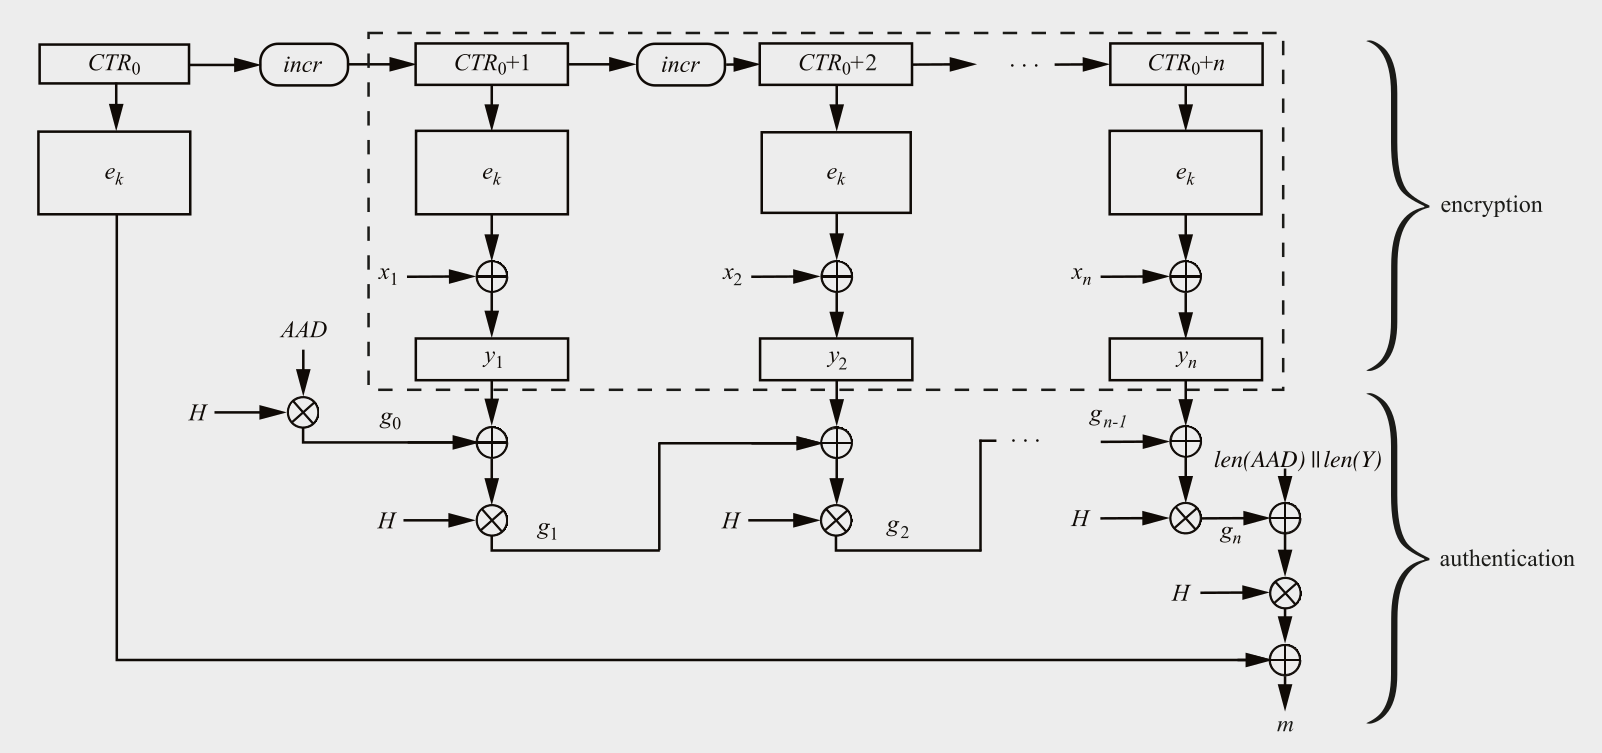
\includegraphics[width=\linewidth,height=0.88\textheight,keepaspectratio]{img/gcm.png}
    \end{center}
\end{frame}

\begin{frame}{GCM: Detalhes e GMAC}
    \textbf{Sobre o GCM:}
    \begin{itemize}
        \footnotesize
        \item As multiplicações são em $GF(2^{128})$ com $P(x) = x^{128} + x^7 + x^2 + x + 1$ $\Rightarrow$ exige cifra de \textbf{bloco de 128 bits} (ex.: AES).
        \item Apenas \emph{uma} multiplicação por bloco $\Rightarrow$ custo de autenticação muito baixo.
        \item Por ligar os dados associados (AAD) ao ciphertext, detecta ataques de ``recombinação'' de cabeçalhos.
    \end{itemize}
    \bigskip
    \textbf{GMAC, a variante ``só MAC'':}
    \begin{itemize}
        \footnotesize
        \item É o GCM \alert{sem cifragem}: computa \emph{apenas} o código de autenticação.
        \item Para aplicações que precisam de integridade/autenticidade, mas \emph{não} de confidencialidade.
        \item Altamente \textbf{paralelizável} $\Rightarrow$ eficiente em hardware: throughputs de \textbf{100 Gbit/s ou mais}.
        \item Padronizado e usado no \textbf{IPsec} (ESP e \textit{Authentication Header}).
    \end{itemize}
\end{frame}

%%%%%%%%%%%%%%%%%%%%%%%%%%%%%%%%%%%
\section{Lições Aprendidas}

\begin{frame}{Lições Aprendidas}
    \begin{itemize}
        \item MACs fornecem \textbf{dois serviços de segurança}: \emph{integridade} e \emph{autenticação} de mensagem, usando técnicas \textbf{simétricas}. São amplamente usados em protocolos práticos.
        \medskip
        \item Esses serviços também são oferecidos por assinaturas digitais, mas MACs são \textbf{muito mais rápidos} (algoritmos simétricos).
        \medskip
        \item MACs \alert{não fornecem não repúdio} (a chave é compartilhada).
        \medskip
        \item MACs de relevância prática baseiam-se em \textbf{cifras de bloco} ou em \textbf{funções hash}.
        \medskip
        \item \textbf{HMAC} é um MAC popular baseado em hash, com prova de segurança; muito usado (TLS, IPsec). \textbf{KMAC} é o equivalente nativo do SHA-3: chaveado por construção, com saída de tamanho variável e separação de domínio embutidas.
        \medskip
        \item \textbf{Encriptação autenticada} (CCM, GCM) entrega confidencialidade \emph{e} autenticação em um passo; \textbf{GMAC} é a variante ``só autenticação'' do GCM.
    \end{itemize}
\end{frame}

\end{document}
